\documentclass[aspectratio=169,10pt]{beamer}
\usetheme{Madrid}
\usecolortheme{whale}

\usepackage[utf8]{inputenc}
\usepackage[spanish,es-nodecimaldot]{babel}
\usepackage{amsmath,amssymb,booktabs,graphicx}
\graphicspath{{../resultados/}{./}}

% Configuración de colores institucionales
\definecolor{externado}{RGB}{140, 20, 20}
\setbeamercolor{palette primary}{bg=externado,fg=white}
\setbeamercolor{structure}{fg=externado}
\setbeamercolor{titlelike}{parent=palette primary}

\title[Proyecto Integrador -- Métodos Numéricos]{Familia Óptima Libre de Derivadas para Raíces Múltiples}
\subtitle{Implementación Computacional, Estabilidad Dinámica, Benchmarking y Extensión Multidimensional}
\author[A. Gómez, J. Duarte, J. Jiménez]{
  Ailyn Sofía Gómez Rodríguez \and Julián Steven Duarte \and Julián Camilo Jiménez Rodríguez
}
\institute[U. Externado]{
  Pregrado en Ciencia de Datos -- Departamento de Matemáticas\\
  \textbf{Universidad Externado de Colombia}\\
  Docente: Edwin Fernando Muñoz Chipatecua
}
\date{Noviembre de 2026}

\begin{document}

% -----------------------------------------------------------------------------
% Diapositiva 1: Portada (20 s)
% -----------------------------------------------------------------------------
\begin{frame}
  \titlepage
\end{frame}

% -----------------------------------------------------------------------------
% Diapositiva 2: El Problema de las Raíces Múltiples (1 min)
% -----------------------------------------------------------------------------
\begin{frame}{1. El Problema: Raíces Múltiples y Régimen de Newton}
  \begin{itemize}
    \item \textbf{Definición de multiplicidad:} Una raíz $\alpha$ tiene multiplicidad $m > 1$ cuando:
    $$g(\alpha) = g'(\alpha) = \dots = g^{(m-1)}(\alpha) = 0, \quad \text{con } g^{(m)}(\alpha) \neq 0$$
    \item \textbf{Régimen de convergencia del método de Newton clásico ($x_{k+1} = x_k - g(x_k)/g'(x_k)$):}
    Para una raíz de multiplicidad $m > 1$, Newton clásico presenta \textbf{convergencia estrictamente lineal}, con factor asintótico de error:
    $$\lim_{k\to\infty} \frac{|x_{k+1}-\alpha|}{|x_k-\alpha|} = \frac{m-1}{m} < 1$$
    \item \textbf{Alternativa clásica y costo computacional:}
    Newton modificado ($x_{k+1} = x_k - m \frac{g(x_k)}{g'(x_k)}$) restaura el orden cuadrático ($p=2$), pero requiere la derivada analítica $g'(x)$, a menudo costosa o inaccesible en problemas prácticos de ciencia de datos.
  \end{itemize}
\end{frame}

% -----------------------------------------------------------------------------
% Diapositiva 3: La Familia de Jerezano et al. (2026) (1 min 30 s)
% -----------------------------------------------------------------------------
\begin{frame}{2. Familia Libre de Derivadas (Jerezano et al., 2026)}
  \begin{block}{Esquema Predictor-Corrector de Dos Pasos}
    \begin{align*}
      w_k &= x_k + \beta [g(x_k)]^2, \quad \beta \in \mathbb{R}\setminus\{0\}\\
      D_k &= g[w_k, x_k] = \frac{g(w_k) - g(x_k)}{w_k - x_k} \quad \text{(secante con paso cuadrático)}\\
      y_k &= x_k - m \frac{g(x_k)}{D_k}\\
      t_k &= \left(\frac{g(y_k)}{g(x_k)}\right)^{1/m} = \exp\left(\frac{1}{m}\operatorname{Log}\left(\frac{g(y_k)}{g(x_k)}\right)\right) \quad \text{con } \operatorname{Arg}(z)\in(-\pi, \pi]\\
      x_{k+1} &= x_k - m H(t_k) \frac{g(x_k)}{D_k}
    \end{align*}
  \end{block}
  \begin{itemize}
    \item \textbf{Condiciones Teorema 2 (Orden 4):} $H(0)=1, \quad H'(0)=1, \quad H''(0)=4, \quad \text{y} \quad |H'''(0)| < \infty$.
    \item \textbf{Variante M1 (Polinomial):} $H_1(t) = 1 + t + 2t^2 \implies H_1'''(0) = 0 < \infty$.
    \item \textbf{Variante M2 (Racional):} $H_2(t) = \frac{1-t}{1-2t} \implies H_2'''(0) = 24 < \infty$ \quad (Polo en $t = 1/2$).
    \item \alert{\textbf{Nota de implementación:}} En aritmética finita, $w_k = x_k$ puede ocurrir por absorción numérica de la perturbación $\beta g(x_k)^2$. La rama principal del logaritmo asegura cálculo univaluado en $\mathbb{C}$, reconociendo su corte de rama.
  \end{itemize}
\end{frame}

% -----------------------------------------------------------------------------
% Diapositiva 4: Optimalidad de Kung-Traub (1 min)
% -----------------------------------------------------------------------------
\begin{frame}{3. Conjetura y Optimalidad de Kung-Traub}
  \begin{columns}
    \column{0.55\textwidth}
    \begin{block}{Conjetura de Kung-Traub (1974)}
      El orden máximo de convergencia de un método multipaso sin memoria con $d$ evaluaciones funcionales por ciclo es:
      $$p \le 2^{d-1}$$
    \end{block}
    \begin{itemize}
      \item La familia evalúa exactamente 3 funciones escalares ($g(x_k), g(w_k), g(y_k)$) y \textbf{cero derivadas} ($d=3$).
      \item Cota máxima teórica: $p \le 2^{3-1} = 4$.
      \item Bajo las condiciones del Teorema 2, la familia alcanza orden cuatro y \textbf{satura la cota de Kung-Traub}.
    \end{itemize}
    \column{0.45\textwidth}
    \textbf{Índice de Eficiencia Teórica ($\mathcal{I} = p^{1/d}$):}
    \begin{table}
      \centering\small
      \begin{tabular}{lccc}
        \toprule
        Método & $p$ & $d$ & $\mathcal{I}$ \\
        \midrule
        Newton estándar & 1 & 2 & 1.000 \\
        Newton modificado & 2 & 2 & 1.414 \\
        Steffensen mod. & 2 & 2 & 1.414 \\
        \textbf{Familia M1 / M2} & \textbf{4} & \textbf{3} & \textbf{1.587} \\
        \bottomrule
      \end{tabular}
    \end{table}
    \vspace{0.1cm}
    \begin{alertblock}{Precisión conceptual}
      $\mathcal{I}$ es una medida teórica basada en orden y evaluaciones; no implica necesariamente menores tiempos de ejecución en una implementación concreta.
    \end{alertblock}
  \end{columns}
\end{frame}

% -----------------------------------------------------------------------------
% Diapositiva 5: Dinámica Compleja y Planos de Estabilidad (1 min 15 s)
% -----------------------------------------------------------------------------
\begin{frame}{4. Estabilidad y Dinámica Compleja en $\mathbb{C}$ (Sección 3)}
  \begin{columns}
    \column{0.5\textwidth}
    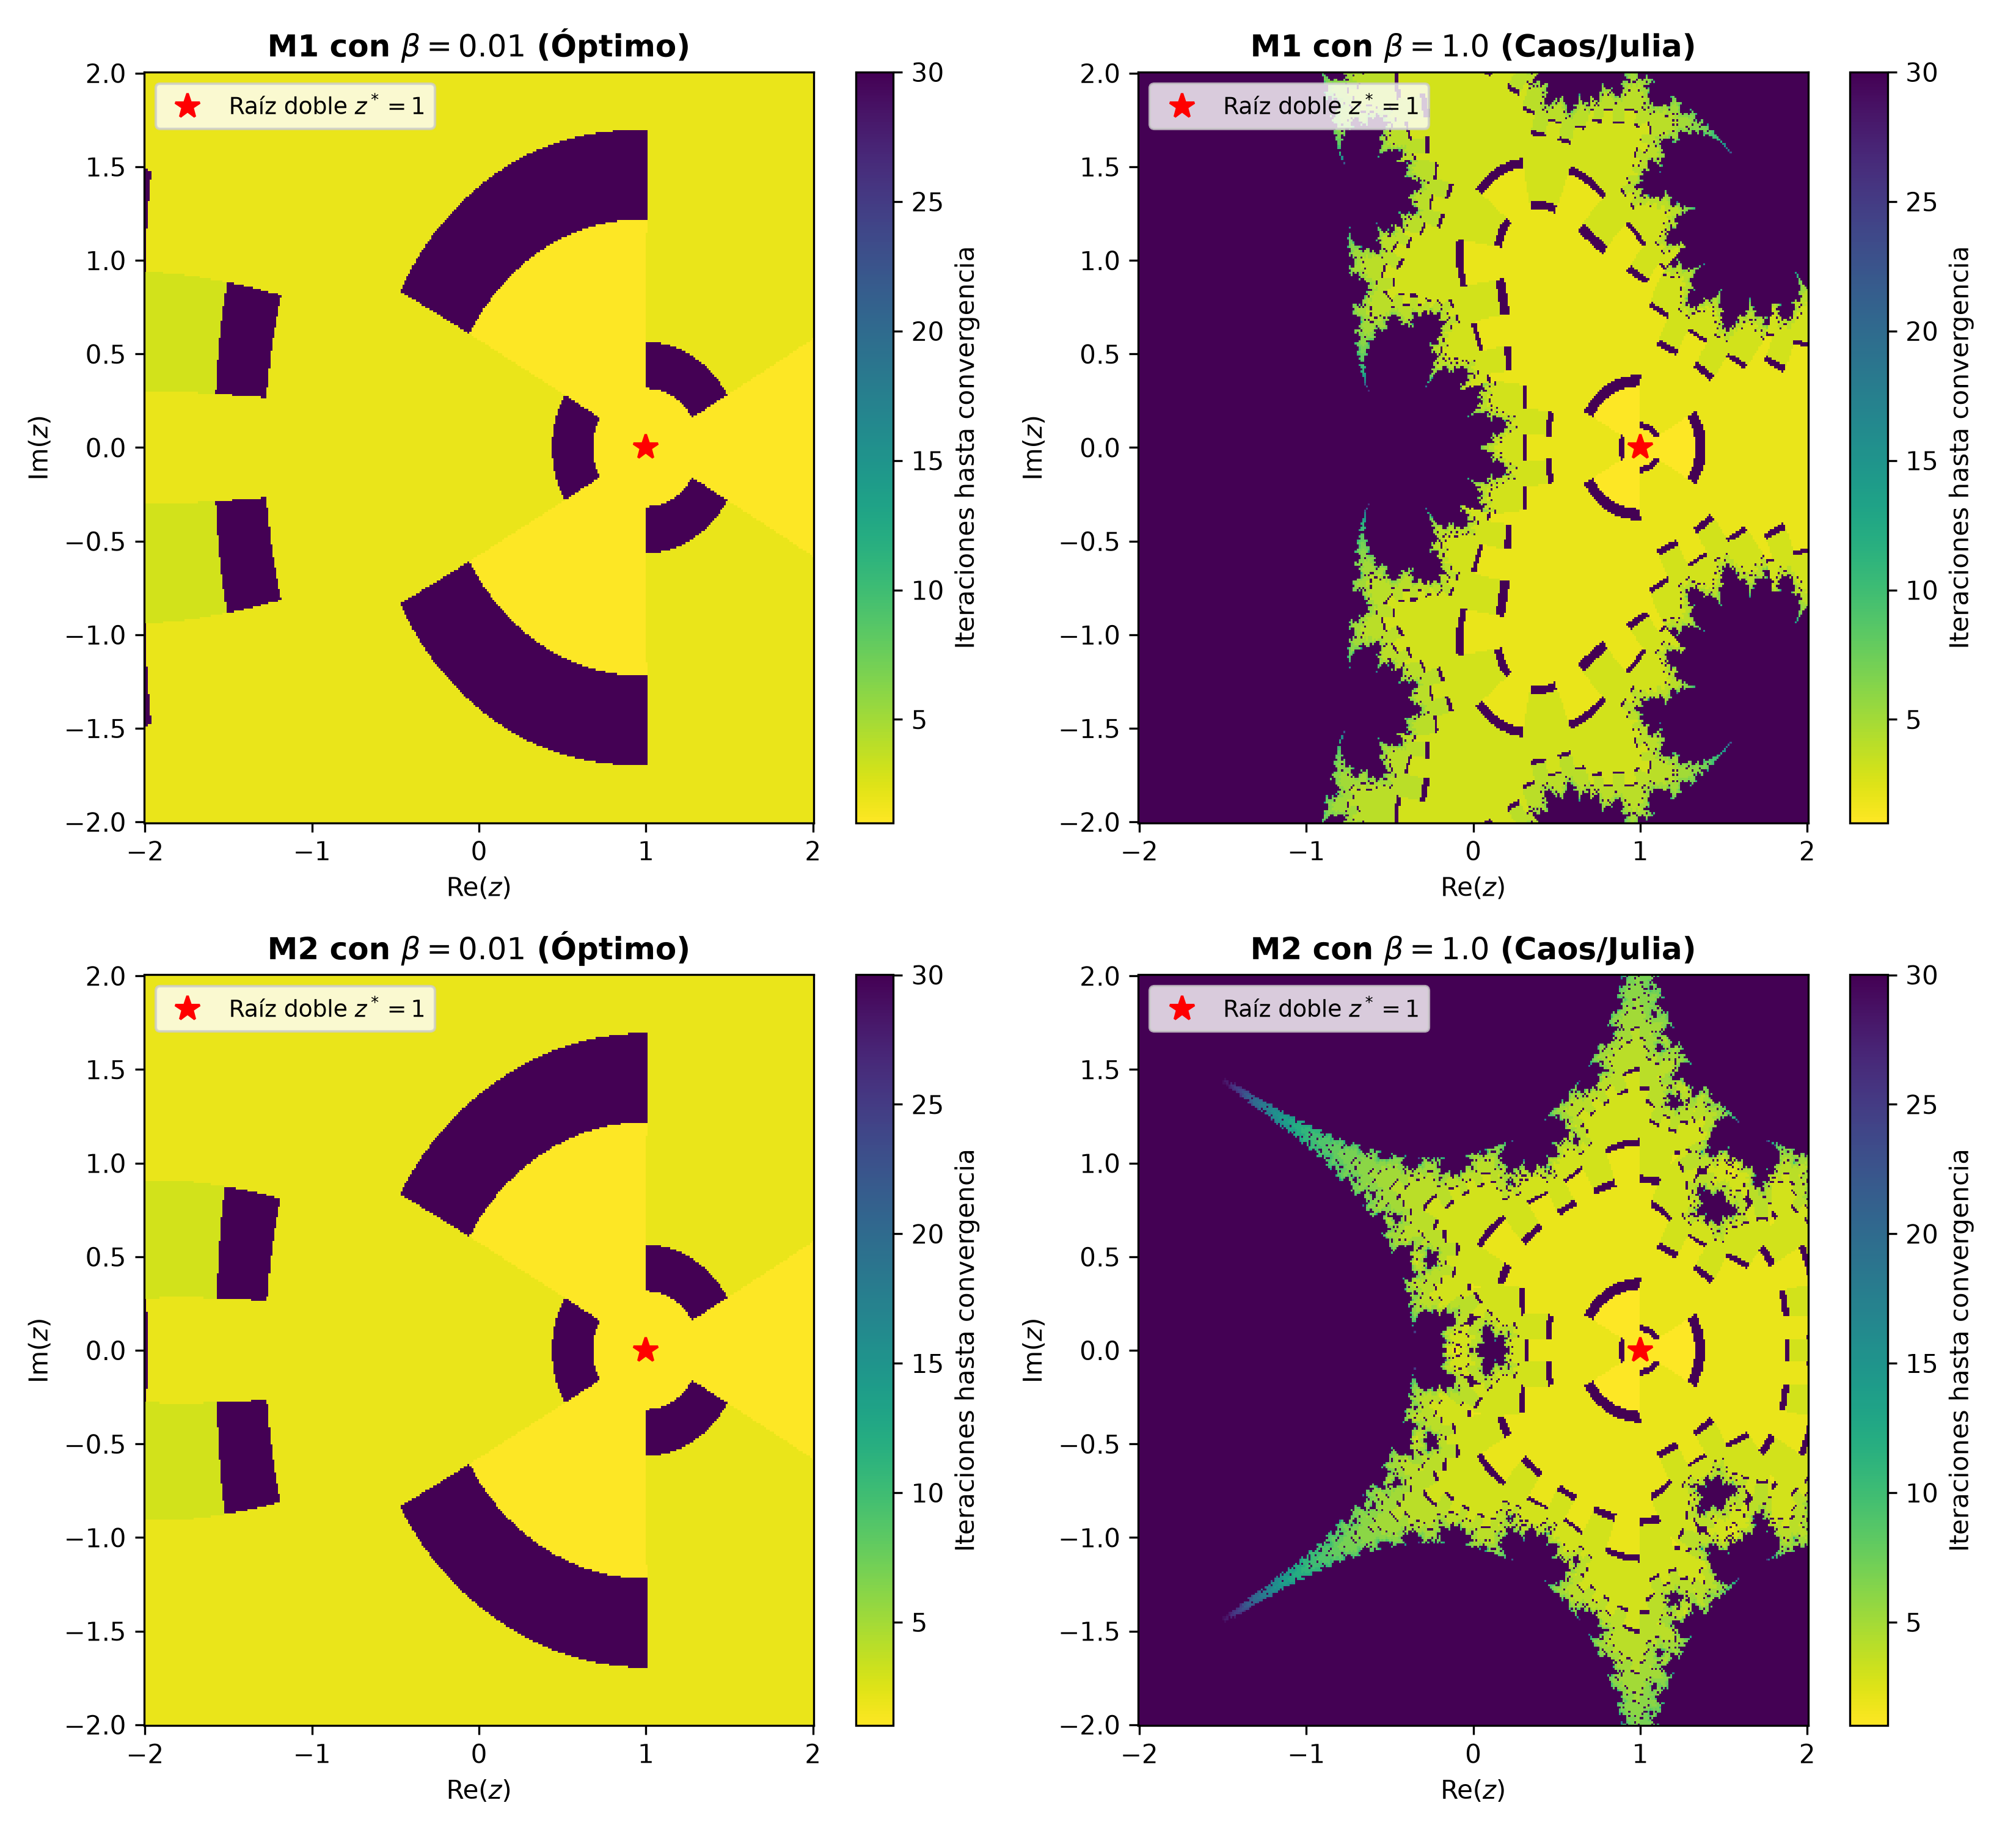
\includegraphics[width=\textwidth]{dinamica_compleja_m1_m2.png}
    \column{0.5\textwidth}
    \begin{itemize}
      \item \textbf{Polinomio Canónico:} $p(z)=(z-1)^2$ ($m=2$).
      \item \textbf{Operador Racional:} $z_{k+1} = R(z, \beta)$. En la raíz $z^*=1$:
      $$R'(1, \beta) = 0 \implies \text{\textbf{Punto fijo superatractor}}$$
      Garantiza convergencia local de orden superior en su vecindad.
      \item \textbf{Observación en la malla examinada ($350\times 350$, máx. 30 iter.):}
      \begin{itemize}
        \item Con $\beta=0.01$, una mayor proporción de puntos alcanza el criterio de convergencia en la malla examinada, según los resultados obtenidos.
        \item Con $\beta=1.0$, se incrementan los puntos sin converger en 30 pasos.
      \end{itemize}
      \item \alert{Rigor:} El ensayo delimita cuencas numéricas finitas; no constituye una caracterización analítica completa de conjuntos de Fatou y Julia.
    \end{itemize}
  \end{columns}
\end{frame}

% -----------------------------------------------------------------------------
% Diapositiva 6: Metodología Computacional y Precisión Finita (1 min)
% -----------------------------------------------------------------------------
\begin{frame}{5. Metodología Computacional y Manejo de Patologías}
  \begin{itemize}
    \item \textbf{Aritmética de Alta Precisión:} \texttt{mpmath} con 150 dígitos decimales (\texttt{dps = 150}) y constantes decimales desde texto para eliminar sesgos binarios.
    \item \textbf{Rama Principal del Logaritmo Complejo:}
    $$t_k = \exp\left(\frac{1}{m}\operatorname{Log}\left(\frac{g(y_k)}{g(x_k)}\right)\right), \quad \operatorname{Arg}(z)\in(-\pi,\pi]$$
    Establece una convención consistente para evaluar $t_k$ en etapas transitorias cuando $g(y)/g(x) < 0$, reconociendo la discontinuidad del corte de rama sobre el semieje real negativo.
    \item \textbf{Criterio de Parada Dual Estricto:} Exigencia simultánea en paso y residuo:
    $$|\Delta x_k| = |x_{k+1}-x_k| < 10^{-25} \quad \wedge \quad |g(x_{k+1})| < 10^{-25}$$
    \item \textbf{Mecanismo de Absorción Numérica (\texttt{Estancamiento w=x}):}
    Cuando la perturbación $\beta g(x_k)^2$ es tan pequeña que, al sumarse a $x_k$, la aritmética de precisión finita produce el mismo valor representable, el código detecta $w_k = x_k$ y detiene controladamente la corrida por imposibilidad de formar la secante.
  \end{itemize}
\end{frame}

% -----------------------------------------------------------------------------
% Diapositiva 7: Resultados Experimentales y Contraste (1 min 30 s)
% -----------------------------------------------------------------------------
\begin{frame}{6. Resultados Experimentales (150 dígitos, $\mathrm{TOL}=10^{-25}$, $\beta=0.01$)}
  \begin{table}
    \centering\scriptsize
    \resizebox{\textwidth}{!}{
    \begin{tabular}{llrrrrrrrrl}
      \toprule
      Problema & Método & Iter. & $g$ eval. & $g'$ eval. & Error abs. & $|\Delta x_k|$ & Residuo & ACOC & $T$ (ms) & Estado \\
      \midrule
      $g_1$, $x_0=1.9$ & M1 & 5 & 17 & 0 & $1.32\times10^{-35}$ & $9.51\times10^{-66}$ & $5.26\times10^{-72}$ & 8.81 & 1.7 & Convergió \\
      $g_1$, $x_0=1.9$ & M2 & 4 & 14 & 0 & $2.03\times10^{-50}$ & $4.14\times10^{-14}$ & $1.24\times10^{-101}$ & -- & 1.3 & Estancamiento $w=x$ \\
      $g_1$, $x_0=1.9$ & Newton mod. & 8 & 10 & 8 & $1.69\times10^{-57}$ & $1.01\times10^{-29}$ & $8.58\times10^{-116}$ & 2.00 & 1.1 & Convergió \\
      $g_1$, $x_0=1.9$ & Steffensen & 8 & 18 & 0 & $1.77\times10^{-57}$ & $1.03\times10^{-29}$ & $9.43\times10^{-116}$ & 2.00 & 1.4 & Convergió \\
      $g_1$, $x_0=1.9$ & KK & 4 & 15 & 0 & $1.01\times10^{-53}$ & $6.83\times10^{-15}$ & $3.06\times10^{-108}$ & -- & 1.5 & Pendiente secante nula \\
      \midrule
      $g_2$, $x_0=5.3$ & Newton mod. & 5 & 7 & 5 & $1.45\times10^{-71}$ & $2.83\times10^{-35}$ & $2.18\times10^{-215}$ & 2.00 & 0.9 & Convergió \\
      $g_2$, $x_0=5.3$ & KK & 3 & 11 & 0 & $9.91\times10^{-117}$ & $9.65\times10^{-29}$ & $7.01\times10^{-351}$ & 3.97 & 1.1 & Convergió \\
      \midrule
      $g_3$, $x_0=2.8$ & M1 & 3 & 11 & 0 & $3.71\times10^{-18}$ & $5.62\times10^{-60}$ & $1.52\times10^{-68}$ & -- & 1.6 & \alert{Criterio dual; error $>$ TOL} \\
      $g_3$, $x_0=2.8$ & M2 & 3 & 11 & 0 & $5.42\times10^{-19}$ & $4.19\times10^{-123}$ & $6.89\times10^{-72}$ & -- & 1.6 & \alert{Criterio dual; error $>$ TOL} \\
      \bottomrule
    \end{tabular}}
  \end{table}
  \vspace{-0.15cm}
  {\tiny \textit{Nota: Se muestran casos representativos; el CSV contiene las corridas completas. El conteo $1+3k+1$ aplica específicamente a M1 y M2 ($g(x_0)$ inicial, $3k$ en pasos y llamada final de verificación $g(x_{\mathrm{final}})$ post-bucle).}}
  \begin{itemize}
    \item \textbf{Contraste con el artículo base:} En $g_1$ ($x_0=1.9$), M1 satisface nuestro criterio dual en 5 iteraciones, frente a las 7 reportadas en el artículo. Esta diferencia no demuestra mayor eficiencia: usamos 150 dígitos y una tolerancia menos estricta ($10^{-25}$) que la configuración original ($10^{-200}$ con 4000 dígitos).
  \end{itemize}
\end{frame}

% -----------------------------------------------------------------------------
% Diapositiva 8: Análisis Crítico de g3 y Validación de ACOC (1 min)
% -----------------------------------------------------------------------------
\begin{frame}{7. Hallazgo en $g_3$ ($m=4$) y Comportamiento del ACOC}
  \begin{columns}
    \column{0.52\textwidth}
    \begin{block}{Terminación vs. Precisión Efectiva en $g_3$}
      \begin{itemize}
        \item Cerca de $\alpha=3$, $g_3(x) \approx -80(x-3)^4$.
        \item Un error de $10^{-18}$ produce un residuo de orden $(10^{-18})^4 \approx 10^{-72}$.
        \item El paso colapsa ($|\Delta x_3| < 10^{-59}$) y cumple operativamente el criterio dual en 3 iteraciones.
        \item \alert{\textbf{Honestidad técnica:}} Como el error real frente a $\alpha=3$ supera $10^{-25}$, no se declara convergencia plena sino terminación anticipada por criterio dual.
      \end{itemize}
    \end{block}
    \column{0.48\textwidth}
    \begin{block}{Orden Computacional Aproximado (ACOC)}
      $$\mathrm{ACOC} \approx \frac{\ln(|\Delta x_{k+1}|/|\Delta x_k|)}{\ln(|\Delta x_k|/|\Delta x_{k-1}|)}$$
      \begin{itemize}
        \item \textbf{Validación canónica ($x^3-x-2=0$):}
        Newton: $\mathrm{ACOC}\approx 2.0000$; secante: $\mathrm{ACOC}\approx 1.6162$, cercano al orden teórico de la razón áurea ($1.6180$).
        \item \textbf{Límite en raíces múltiples:} Con pocas iteraciones (3 a 5), la drástica contracción distorsiona el cociente logarítmico (ej. 8.81 en M1), lo que no prueba orden superior a cuatro.
      \end{itemize}
    \end{block}
  \end{columns}
\end{frame}

% -----------------------------------------------------------------------------
% Diapositiva 9: Experimento Multidimensional: Broyden (1 min)
% -----------------------------------------------------------------------------
\begin{frame}{8. Extensión a Sistemas No Lineales $2\times 2$ (Semana 9)}
  \begin{itemize}
    \item Para ilustrar esquemas sin derivadas en varias dimensiones, resolvemos:
    $$\mathbf{F}(x_1, x_2) = \begin{pmatrix} x_1^2 + x_2^2 - 4 \\ x_1 x_2 - 1 \end{pmatrix} = \mathbf{0}, \quad \text{con semilla } \mathbf{x}_0 = (1.5, 0.8)^T$$
  \end{itemize}
  \begin{table}
    \centering\small
    \begin{tabular}{lcccc}
      \toprule
      Método & Iteraciones & Sistemas lineales resueltos & Evaluaciones derivadas & Residuo final \\
      \midrule
      Newton Multivariable & 5 & 5 densos & 20 entradas Jacobianas & $3.92\times 10^{-15}$ \\
      Secante Multivariable (Broyden) & 10 & 10 densos & 0 derivadas analíticas & $4.25\times 10^{-15}$ \\
      \bottomrule
    \end{tabular}
  \end{table}
  \begin{block}{Compromiso Computacional y Costo Operativo}
    Broyden actualiza la aproximación del Jacobiano mediante una corrección de rango uno con costo $O(n^2)$ y evita calcular $n^2$ derivadas analíticas, aunque la resolución de sistemas densos continúa teniendo un costo de orden $O(n^3)$ por iteración.
  \end{block}
\end{frame}

% -----------------------------------------------------------------------------
% Diapositiva 10: Conexión con Ciencia de Datos y Optimización (40 s)
% -----------------------------------------------------------------------------
\begin{frame}{9. Conexión con Ciencia de Datos y Optimización}
  \begin{columns}
    \column{0.55\textwidth}
    \textbf{Condición de optimalidad de primer orden:}
    $$\nabla L(\boldsymbol{\theta}) = \mathbf{0}$$
    \begin{itemize}
      \item En Machine Learning, el entrenamiento busca puntos estacionarios de funciones de pérdida complejas.
      \item En regiones mal condicionadas, la Hessiana puede presentar autovalores cercanos a cero, lo que dificulta ciertos métodos de optimización.
      \item Estos escenarios motivan estudiar puntos críticos degenerados, aunque una Hessiana singular no implica necesariamente una raíz de multiplicidad $m>1$.
    \end{itemize}
    \column{0.45\textwidth}
    \begin{block}{Relevancia Metodológica}
      Los métodos estudiados ofrecen una referencia teórica para investigar algoritmos que aprovechen información sobre multiplicidad. Su aplicación a pérdidas de alta dimensión requiere extensiones y validaciones adicionales.
    \end{block}
  \end{columns}
\end{frame}

% -----------------------------------------------------------------------------
% Diapositiva 11: Conclusiones y Trabajo Futuro (50 s)
% -----------------------------------------------------------------------------
\begin{frame}{10. Conclusiones y Trabajo Futuro}
  \begin{itemize}
    \item \textbf{Implementación algorítmica:} Se implementó una familia de métodos cuyo orden teórico es cuatro y que alcanza la cota de Kung-Traub bajo las condiciones establecidas por el artículo, documentando tanto casos convergentes como estancamientos controlados.
    \item \textbf{Criterio científico en benchmarking:} Se corrigieron interpretaciones en $g_3$, distinguiendo la terminación por criterio dual de la precisión efectiva frente a la raíz.
    \item \textbf{Comportamiento dinámico:} En la malla y el límite de iteraciones examinados, $\beta=0.01$ mostró un comportamiento de convergencia más favorable que $\beta=1.0$.
    \item \textbf{Limitaciones:} El método asume conocida la multiplicidad exacta $m$.
    \item \textbf{Trabajo futuro:}
    \begin{enumerate}
      \item Diseñar estimadores dinámicos de $m$ durante las iteraciones iniciales.
      \item Explorar extensiones libres de derivadas para optimización en problemas de mayor dimensión.
    \end{enumerate}
  \end{itemize}
  \vspace{0.2cm}
  \centering
  \textbf{¡Muchas gracias por su atención! Abrimos la sesión de preguntas y discusión.}
\end{frame}

\end{document}
